% Metódy inžinierskej práce

\documentclass[10pt,twoside,slovak,a4paper]{article}

\usepackage[slovak]{babel}
%\usepackage[T1]{fontenc}
\usepackage[IL2]{fontenc} % lepšia sadzba písmena Ľ než v T1
\usepackage[utf8]{inputenc}
\usepackage{graphicx}
\usepackage{url} % príkaz \url na formátovanie URL
\usepackage{hyperref} % odkazy v texte budú aktívne (pri niektorých triedach dokumentov spôsobuje posun textu)

\usepackage{cite}
%\usepackage{times}

\pagestyle{headings}

\title{Rôzné Metódy a Výhody Gamifikácie Profesionálnych a Každodenných Úloh na Príklade Habitica\thanks{Semestrálny 
projekt v predmete Metódy inžinierskej práce, ak. rok 2022/23, vedenie: Ing. Fedor Lehocki, PhD.}} 
% meno a priezvisko vyučujúceho na cvičeniach

\author{Danylo Tokarskyi\\[2pt]
	{\small Slovenská technická univerzita v Bratislave}\\
	{\small Fakulta informatiky a informačných technológií}\\
	{\small \texttt{xtokarskyi@stuba.sk}}
	}

\date{\small 6. 11. 2022 } % upravte



\begin{document}

\maketitle

\begin{abstract}
	Článok bude o rôznych druhoch gamifikácie, metódach, ich typoch, a ako sa všetci spájajú, aby zvýšili efektivitu 
	vykonania úloh a motiváciu k tomu v profesionálnom a každodennom živote. Habitica, aplikácia pre mobilné telefóny 
	navrhnutá tak, aby pomohla gamifikovať úlohy tým, že si za ich splnenie po-skytne virtuálne výhody a veci, okrem 
	iného, bude použitá ako príklad toho,ako sa dajú tieto metódy využiť, kombinovať a aké výhody to môže priniesť.
	Na potvrdenie ich u¾itoènosti budú zahrnuté štatistické a iné údaje z rôznychzdrojov.
\end{abstract}



\section{Úvod}

Gamifikácia vo všeobecnosti označuje technologický, ekonomický, kultúrny a spoločenský vývoj, v 
ktorom sa realita stáva hravejšou, a teda vo väčšej miere si môže dovoliť získavanie zručností, 
motivačných výhod, kreativity, hravosti, angažovanosti a celkovo pozitívneho rastu a šťastia. 
Všetky tieto aspekty sú bežne vnímané ako pozitívne výhody hry a hrania hier.\cite{Gamification}

Sa bude diskutovať o metódach a výhodách gamifikácie. 
V prvej časti bude 
uvedená všeobecná definícia 
gamifikácie\ref{definition}. Ďalej budú opísané rôzne metódy gamifikácie 
a ich príklady uvedené v Habitica\ref{methods}. 
Potom sa ukážu štatistické údaje o tom, či gamifikácia 
prináša nejaké výhody\ref{benefits}.



\section{Všeobecná definícia} \label{definition}

Gamifikácia je strategický pokus o zlepšenie systémov, služieb, organizácií a činností vytváraním podobných zážitkov, aké sa vyskytujú pri hraní hier, s cieľom motivovať a zaujať používateľov\cite{Gamification}. To sa vo všeobecnosti dosahuje aplikáciou prvkov herného dizajnu a herných princípov (dynamika a mechanika) v neherných kontextoch\cite{Defining}

\section{Metódy} \label{methods}

Gamifikačné techniky sú určené na využitie prirodzených túžob ľudí po socializácii, učení, majstrovstve, súťaži, úspechu, postavení, sebavyjadrení, altruizme alebo uzavretí sa, alebo jednoducho ich reakcii na rámcovanie situácie ako hru alebo hru.\cite{Shallow}

Gamifikáciu možno rozdeliť na dva hlavné typy: gamifikácia založená na odmene a zmysluplná gamifikácia. \cite{Methods}

\subsection{Gamifikácia založená na odmene} \label{methods:reward}
Gamifikácia založená na odmene pozostáva z prvkov gamifikácie, ako sú body, úroveň, tabuľka výsledkov a odznaky.

\cite{Methods} Habitica má úrovne, úspechy, predmety, vybavenie, domáce zvieratá a odmeny.

\subsection{Zmysluplná gamifikácia} \label{methods:meaningful}
Zmysluplná gamifikácia môže odmeňovať používateľov, vyzývať používateľov, prinútiť používateľov ovplyvňovať ostatných a baviť sa a hrať sa. Používateľom tiež dáva možnosť voľby a pocit kontroly a informuje ich o vplyve ich akcií na skutočný svet. To môže spôsobiť, že používatelia budú medzi sebou súťažiť.\cite{Methods}

Habitica má prispôsobenie avatara, štatistiky. Môžete tiež komunikovať s ostatnými hráčmi pomocou cechov, krčiem, večierkov a výziev.

\subsection{Všeobecná interaktivita} \label{methods:interactivity}
Všeobecná interaktivita je nevyhnutným faktorom pre zvýšenie zapojenia používateľov do softvérových aplikácií. Rôzne interakcie, ako je posúvanie, približovanie, klepanie, klikanie a ťahanie, môžu zvýšiť zapojenie používateľov do aplikácií. Výsledkom je, že povzbudzovanie používateľov, aby interagovali s aplikáciou klikaním, neustálym klepaním a presúvaním sa z jednej stránky na druhú v rámci aplikácie, zvýši zapojenie používateľov do aplikácie.\cite{Methods}

Habitica má množstvo rôznych kariet, ponúk a stránok, ku ktorým možno pristupovať posúvaním a ťuknutím

\section{Výhody} \label{benefits}
Ako dôkaz užitočnosti aplikácie použijem prieskum, ktorý uskutočnili Sergio Madera a Pablo Figueroa.\cite{StudyOnPotentialOfVideogames}

\subsection{Metodika experimentu} \label{benefits:methodology}
54 ľudí vyplnilo prieskum určený na meranie ich individuálnej úrovne motivácie k určitému vlastnému strednodobému cieľu. 
Potom bola skupine 27 ľudí predstavená Habitica, videohra navrhnutá tak, aby motivovala ľudí, aby zlepšili svoj život a 
dosiahli svoje ciele; bolo im povedané, aby ho používali aspoň každé dva dni počas dvoch týždňov. 
Všetci účastníci mali možnosť vyhrať ekvivalent 35 dolárov v kolumbijskej mene. Po tomto období 
všetky subjekty vyplnili ďalší prieskum podobný tomu prvému. Väčšina účastníkov boli vysokoškoláci\cite{StudyOnPotentialOfVideogames}

Prieskum pozostáva zo šiestich otázok, z ktorých každá zodpovedá jednému motivačnému meraniu, napríklad 
"Aký náročný bol proces dosiahnutia vášho cieľa" alebo "Aký veľký záujem máte o dosiahnutie svojho cieľa?". 
Väčšina otázok používa 7-bodovú škálu, kde 7 znamená "veľmi veľa" a 1 "veľmi málo" v kontexte otázky.\cite{StudyOnPotentialOfVideogames}

\subsection{Výsledky experimentu} \label{benefits:results}
Obrázok (tabuľky a zodpovedajúce grafy) od 1 do 3 zobrazujú výsledky prieskumných otázok v oboch fázach experimentu. 
"Pred" je fáza, v ktorej ani jedna skupina nepoužívala Habiticu, a 
"Post" fáza, v ktorej ju jedna skupina používala dva týždne.

Vo fáze Post ukazuje obrázok 1 dramatický pokles najvyššieho skóre 
záujmu z kontrolnej skupiny v porovnaní so stabilitou skupiny Habitica.

\begin{figure}[h]
\caption{Tabuľka a graf č. 1}
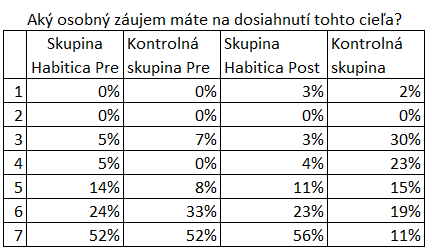
\includegraphics[scale=0.85]{zaujemTable.png}
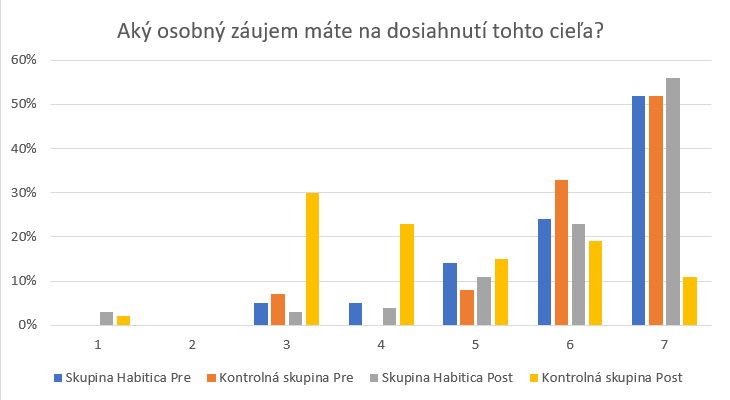
\includegraphics[scale=0.5]{zaujem.png}
\centering
\end{figure}

Pokiaľ ide o fázu Post, obrázok 2 ukazuje významný nárast hodnotení "veľmi dobré" 
o skúsenosti zo skupiny Habitica, zatiaľ čo hodnotenia z kontrolnej skupiny zostávajú stabilné. 
Okrem toho, pre rovnakú fázu, obrázok 3 zobrazuje veľmi dôležité zvýšenie skóre 
výkonnosti zo skupiny Habitica v porovnaní s kontrolnou skupinou.\cite{StudyOnPotentialOfVideogames}

\begin{figure}[h]
	\caption{Tabuľka a graf č. 2}
	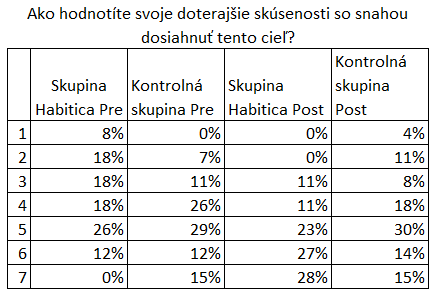
\includegraphics[scale=0.7]{skusenostiTable.png}
	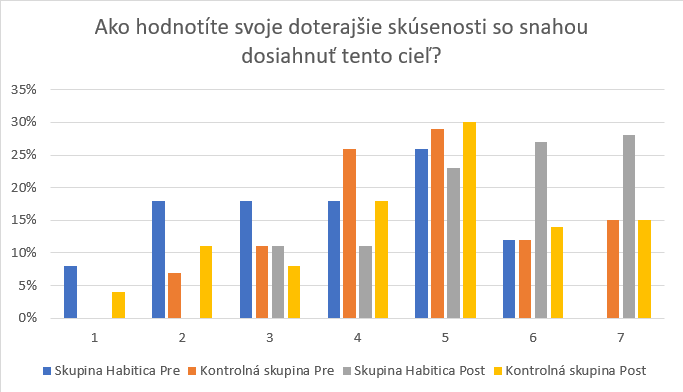
\includegraphics[scale=0.5]{skusenosti.png}
	\centering
\end{figure}
\begin{figure}[h]
	\caption{Tabuľka a graf č. 3}
	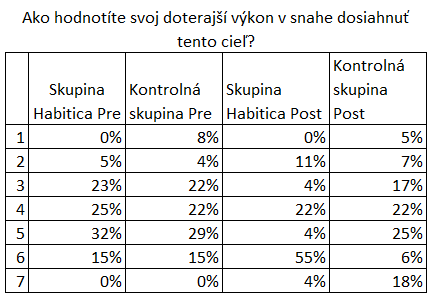
\includegraphics[scale=0.7]{vykonTable.png}
	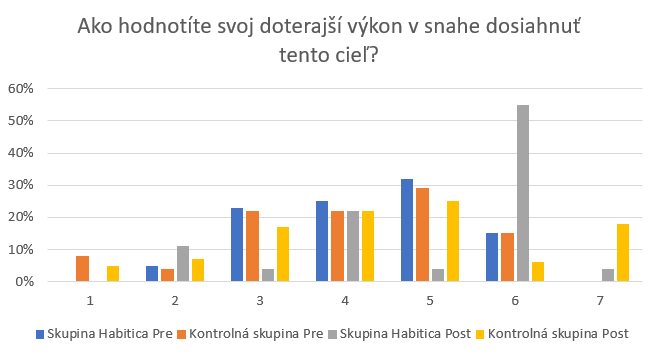
\includegraphics[scale=0.5]{vykon.png}
	\centering
\end{figure}

\section{Záver} \label{conclusion}
Videohry sa stávajú čoraz populárnejším médiom u populácie na celom svete. 
Ich efekty na schopnosť a motiváciu ľudí dosahovať ciele boli dôkladne študované. 
Prevzatie niektorých prvkov videohier a ich uplatnenie v iných sférach ľudskej 
činnosti sa zdá byť schopné zvýšiť ich schopnosť do dosahovaní svojich úloh. 
Je však dôležité poznamenať, že štúdií o gamifikácii nie je príliš veľa, a 
preto nemôžeme úplne zistiť, ako to ovplyvňuje ľudí.

\bibliography{literatura}
\bibliographystyle{plain} % prípadne alpha, abbrv alebo hociktorý iný
\end{document}
